\documentclass[12pt]{article}
\usepackage{natbib}
\usepackage{pgf}
  \bibliographystyle{plainnat}
  \setcitestyle{citesep={,},aysep={}}
\usepackage[colorlinks,citecolor=blue,linkcolor=black,bookmarks=false,hypertexnames=true]{hyperref} 
\usepackage{url}
\usepackage[inline]{enumitem}
\usepackage{float}
\usepackage[bottom,perpage,multiple]{footmisc}
\usepackage{booktabs}
\usepackage{graphicx}
\usepackage{xcolor}
\usepackage{setspace}

\usepackage{enumitem}
\setlist{nosep}

  \setstretch{1.1}
\setlength{\bibsep}{0.0pt}
\tolerance=800

\usepackage{pgfplots}
%\DeclareUnicodeCharacter{2212}{-}
%\usepgfplotslibrary{groupplots,dateplot}
%\usetikzlibrary{patterns,shapes.arrows}
\pgfplotsset{compat=newest}

\usepackage{url}
\renewcommand*{\bibfont}{\footnotesize}

\title{New method to predict patterns' importances}
\author{Aibolit team}
\begin{document}
\maketitle
\newpage

\section*{Previous experiment}
According to last experiments
patterns 'Non final class', 
'Non final attribute', 
'Null check' and 
'Var in the middle' 
are most frequent and important. 

In previous experiment we trained
model without this patterns
and got best distribution of
patterns' importances. 
Our model predict pattern which
has the greatest impact on the
complexity. On the graphics
there is a distribution of 
most important
patterns. 

Results of previous experiment
are on the table (how to change quality
of the model after removing patterns).
\newline
p1 - remove pattern 'Non final class'
\newline
p2 - remove pattern 'Non final attribute'
\newline
p3 - remove pattern 'Null check'
\newline
p4 - remove pattern 'Var in the middle'
\newline

\begin{table}[h] \centering
\begin{tabular}{ | l | l | l | l |} 
	\hline
	Patterns & mse & mae & r2  \\ \hline
	no removing & 0.0182 & 0.0922 &  0.4792 \\ \hline
	p1 & 0.0181 & 0.0922 & 0.4811  \\ \hline
	p2 & 0.0195 & 0.0993 & 0.4395 \\ \hline
	p3 & 0.0209 & 0.1 & 0.4017 \\ \hline
	p4 & 0.0183 & 0.0932 & 0.4763 \\ \hline
	p1, p2 & 0.0196 & 0.0993 & 0.4366 \\ \hline
	p1, p3 & 0.0207 & 0.1 & 0.4052 \\ \hline
	p1, p4 & 0.0185 & 0.0935 & 0.4698 \\ \hline
	p2, p3 & 0.0228 & 0.1085 & 0.3453 \\ \hline
	p2, p4 & 0.02 & 0.1009 &  0.4259 \\ \hline
	p3, p4 & 0.0213 & 0.1016 & 0.3892 \\ \hline
	p1, p2, p3 & 0.0228 & 0.1087 & 0.3467 \\ \hline
	p1, p2, p4 & 0.02 & 0.1013 & 0.4264 \\ \hline
	p1, p3, p4 & 0.0214 & 0.1018 & 0.3874 \\ \hline
	p2, p3, p4 & 0.0235 & 0.1114 & 0.327 \\ \hline
	p1, p2, p3, p4 & 0.0237 & 0.1125 & 0.32 \\ \hline
\end{tabular}
\label{results}
\caption{Results of previous experiment}
\end{table}
\newpage
\section*{New method to predict patterns' importances}
We suggested new method to predict patterns' 
importances. Model is trained on dataset. 
\newline
To predict patterns' importances need to 
do following acts:
\newline
1. Each pattern (in rotation) decreased
(increased) by 1 and predict complexity
for modified snippet. 

Calculate pattern importance as minimum of 
3 complexity for non-modified snippet,
increased by 1 snippet,
decreased by 1 snippet.
\newline
2. sorted importances and 
got necessary ranked array.

\begin{figure}[h!]\center
	\begin{tabular}{cc}
		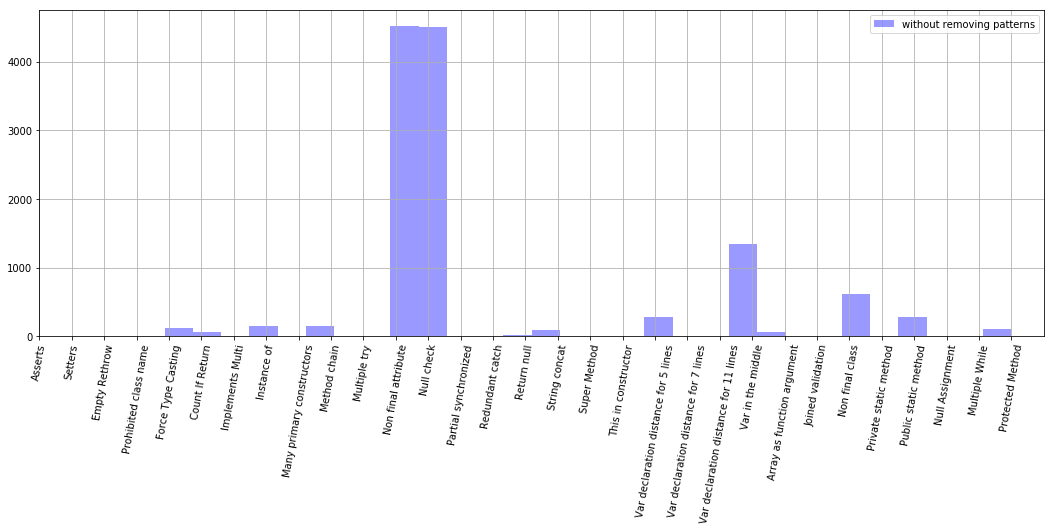
\includegraphics[scale=0.4]{1-2.png}
	\end{tabular}
	\caption{Removing all 4 patterns - old method}
	\label{fig:ris1}
\end{figure}
\begin{figure}[h!]\center
	\begin{tabular}{cc}
		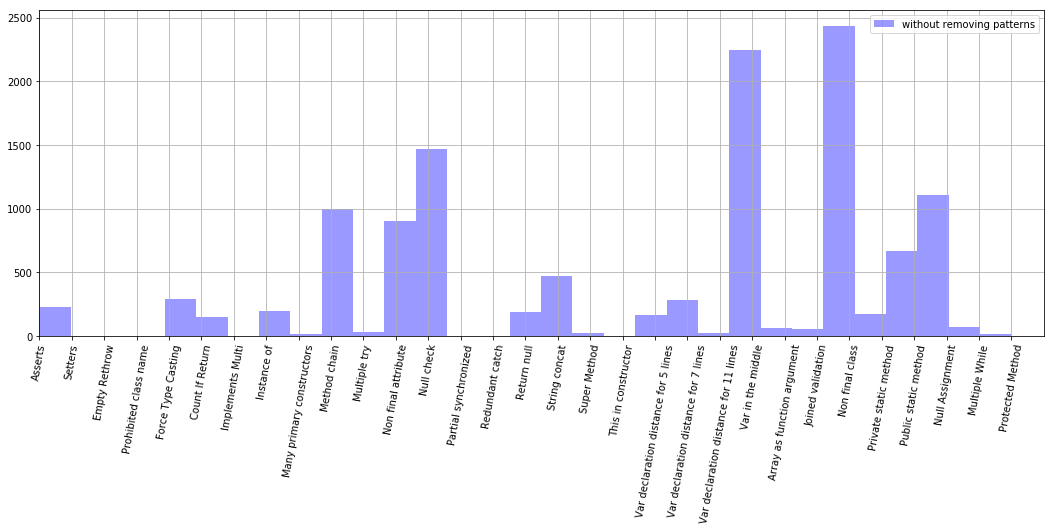
\includegraphics[scale=0.4]{1-1.png}
	\end{tabular}
	\caption{Removing all 4 patterns - new method}
	\label{fig:ris2}
\end{figure}
\newpage
\begin{figure}[h!]\center
	\begin{tabular}{cc}
		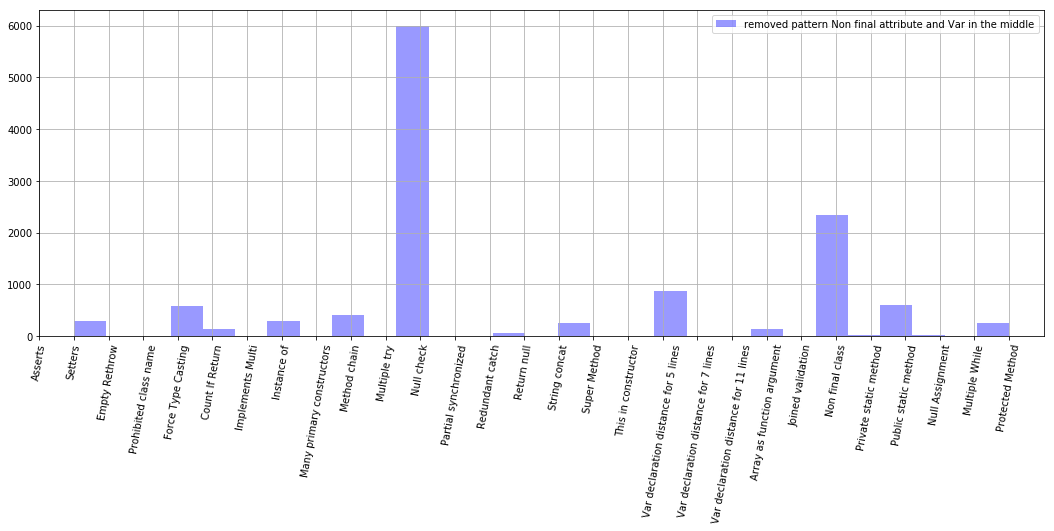
\includegraphics[scale=0.4]{2-2.png}
	\end{tabular}
	\caption{Removing patterns 'Non final attribute' and 'Var in the middle' - old method}
	\label{fig:ris3}
\end{figure}
\begin{figure}[h!]\center
	\begin{tabular}{cc}
		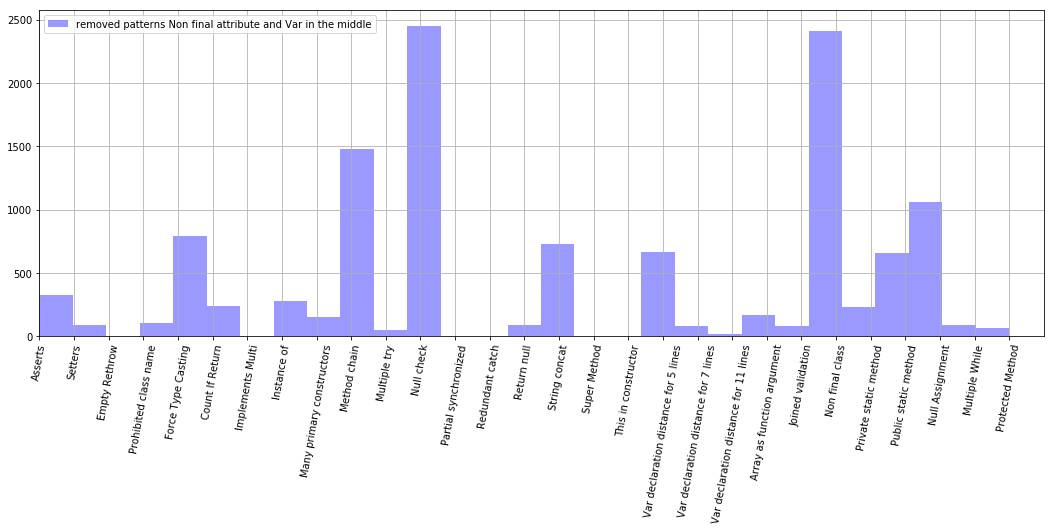
\includegraphics[scale=0.4]{2-1.png}
	\end{tabular}
	\caption{Removing patterns 'Non final attribute' and 'Var in the middle' - new method}
	\label{fig:ris4}
\end{figure}
\newpage
\begin{figure}[h!]\center
	\begin{tabular}{cc}
		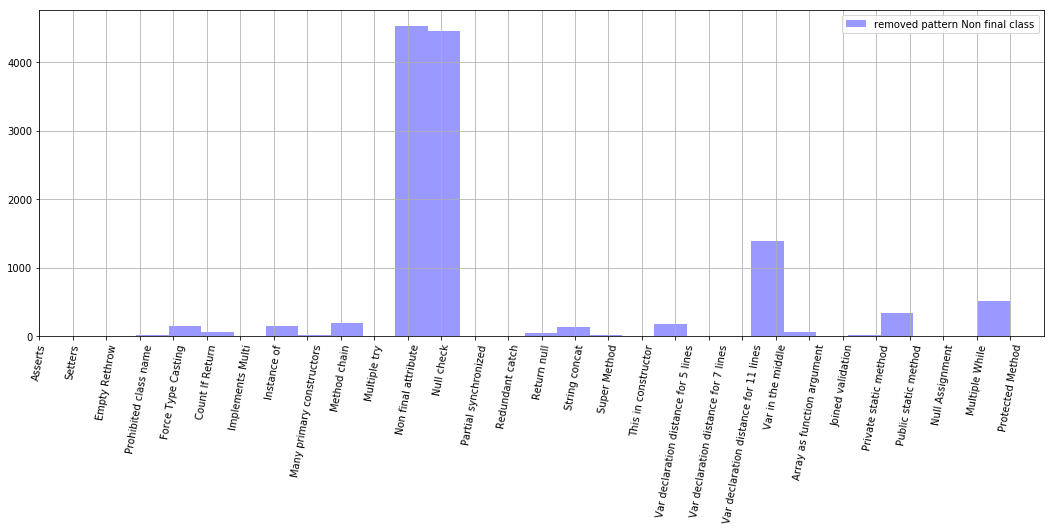
\includegraphics[scale=0.4]{3-2.png}
	\end{tabular}
	\caption{Removing pattern 'Non final class' - old method}
	\label{fig:ris5}
\end{figure}
\begin{figure}[h!]\center
	\begin{tabular}{cc}
		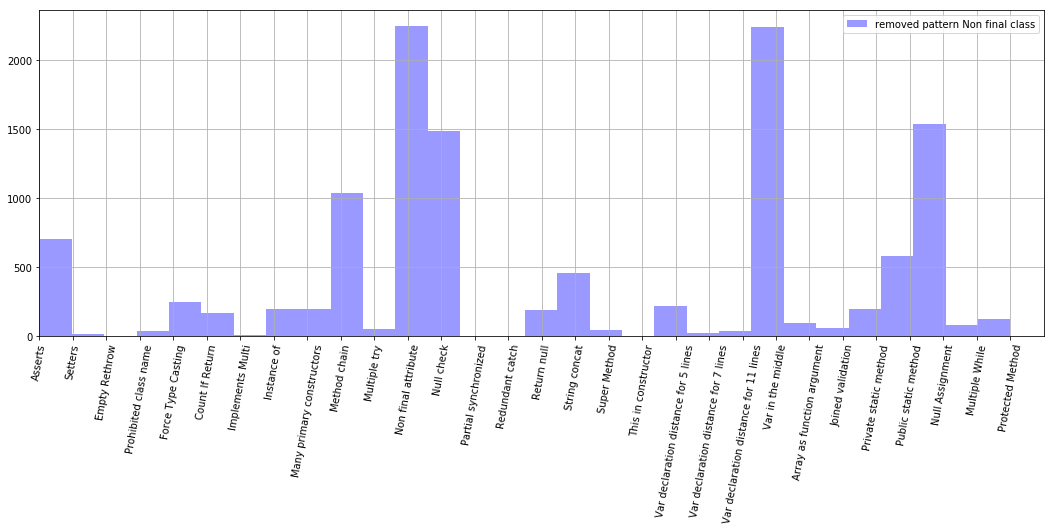
\includegraphics[scale=0.4]{3-1.png}
	\end{tabular}
	\caption{Removing pattern 'Non final class' - new method}
	\label{fig:ris6}
\end{figure}
\newpage
\section*{Comparison of two methods}

According to the graphics in case of 
new method distribution 
of patterns' importances got more balanced.
For each combination of removing patterns 
(from table 1) kl-divergence between
distributions of patterns' importances from
new and old methods was calculated. Results are on the graphic
below.
\begin{figure}[h!]\center
	\begin{tabular}{cc}
		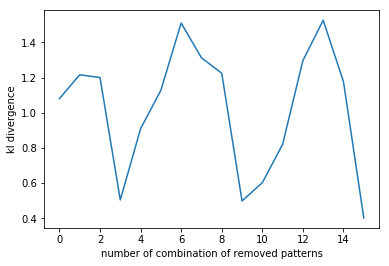
\includegraphics[scale=0.5]{4.png}
	\end{tabular}
	\caption{kl-divergence}
	\label{fig:ris7}
\end{figure}
\newpage
According to the graphic \ref{fig:ris7}
there are significant differences between
distributions.

In case of new method next situation is
probable: all changes doesn't decrease 
complexity. It's undefined behaviour of
this method. So need to choose combinations of 
removing patterns where this mistake are
not significant.

\section*{Conclusion}
In case of 
new method distribution 
of patterns' importances
get more balanced.
Better to use new method
without removing patterns
because then
correlation between
quality of prediction 
complexity, quality of
distribution and count
of described above 
mistakes is optimal. 

 
\end{document}